\documentclass[english,10pt,a4paper]{article}
\usepackage[T1]{fontenc}
\usepackage[left=3cm, right=3cm, top=2cm, bottom=2cm]{geometry}
\usepackage[backend=biber, style=apa]{biblatex} % Example with APA style
\addbibresource{references.bib} % Your bibliography file
\usepackage{graphicx}
\usepackage{float}
\usepackage{mathtools}
\usepackage{amssymb}
\usepackage{amsthm}
\usepackage{babel}
\usepackage{hyperref}
\usepackage{listings} % Package for code formatting
\usepackage{xcolor}    % Colors for syntax highlighting
\usepackage{multirow} % Required for vertical merging
% MATLAB Code Style
\lstdefinestyle{matlab}{
	language=Matlab,
	basicstyle=\ttfamily\footnotesize,
	keywordstyle=\color{blue},
	commentstyle=\color{green!50!black},
	stringstyle=\color{red},
	numbers=left,
	numberstyle=\tiny\color{gray},
	stepnumber=1,
	breaklines=true,
	frame=single
}
\author{Xu Duan \& Benito Ribadeneira}
\title{Robotics Library: Forward and Inverse Kinematics}
\newcommand{\tr}{\text{tr}}
\begin{document}
    \maketitle
    \section{Introduction to Franka Emika Panda}
    Panda is a 7-DoF robot arm. Here is the picture \cite{franka_emika_2017}.
    \begin{figure}[H]\label{joints}
        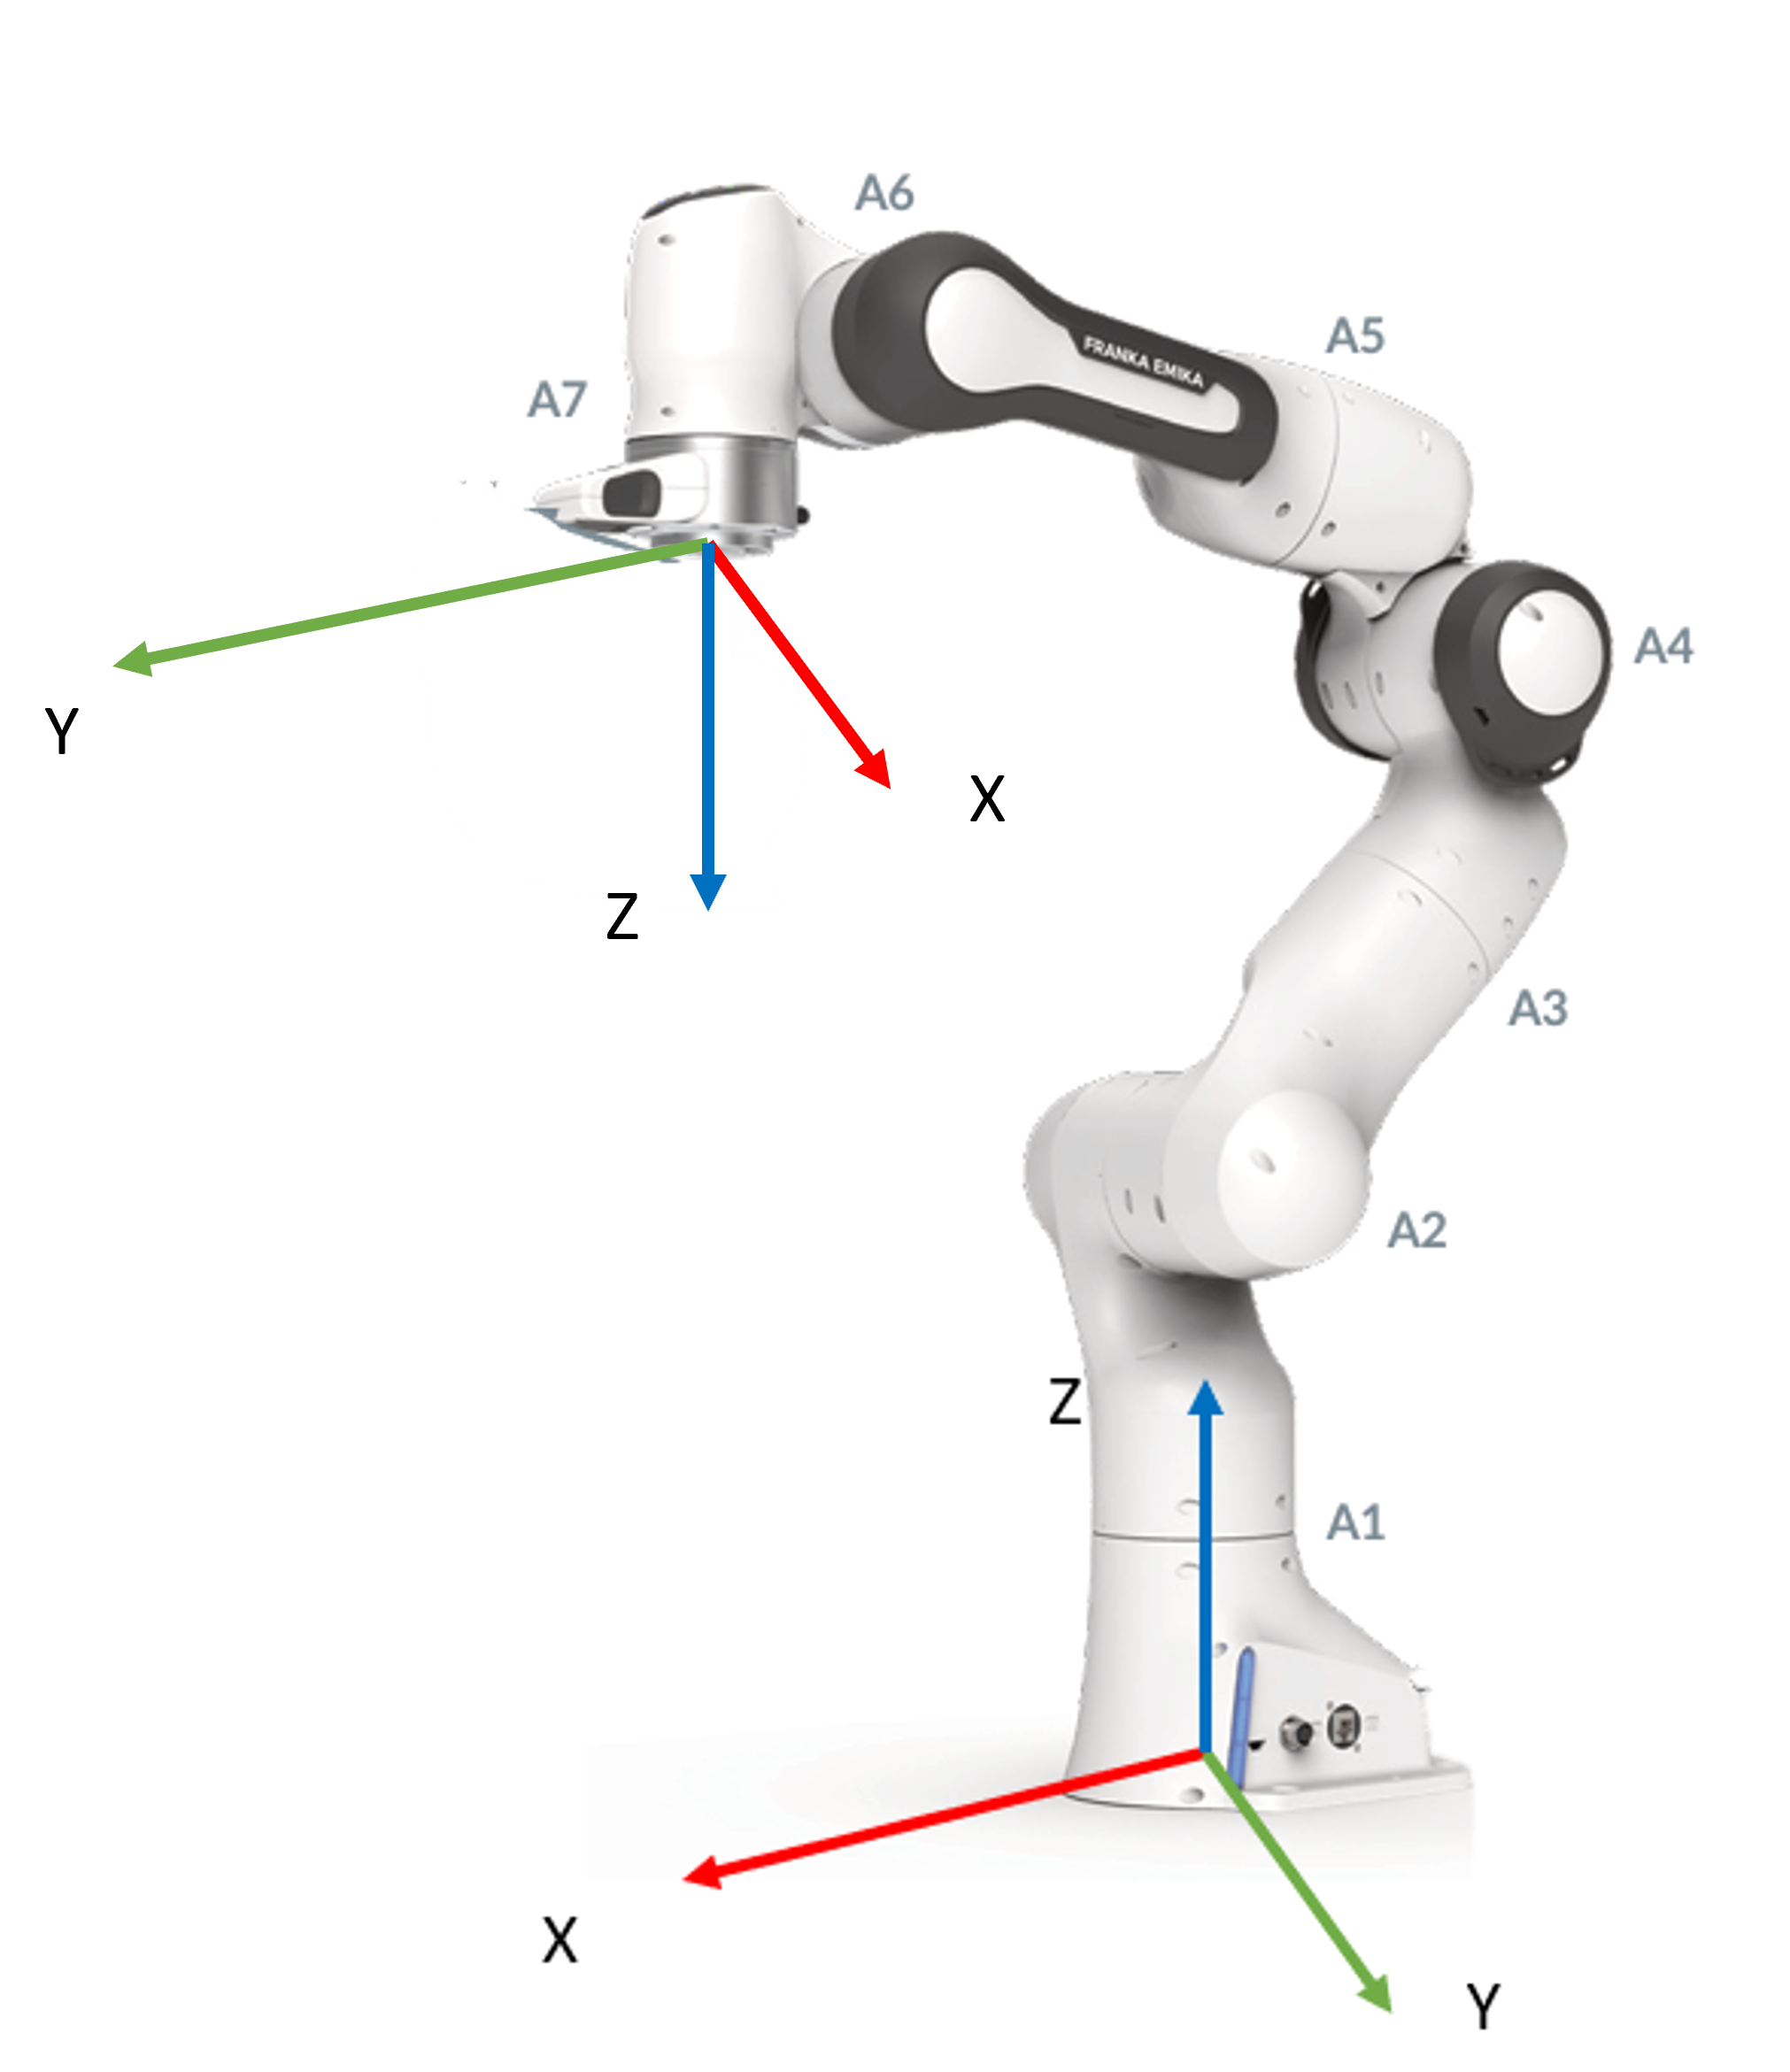
\includegraphics[scale=0.7]{config2.png}
        \caption{The arms and joints of the Panda robot}
    \end{figure}

    Here are the dimensions of the robot.
    \begin{figure}[H]\label{dims}
        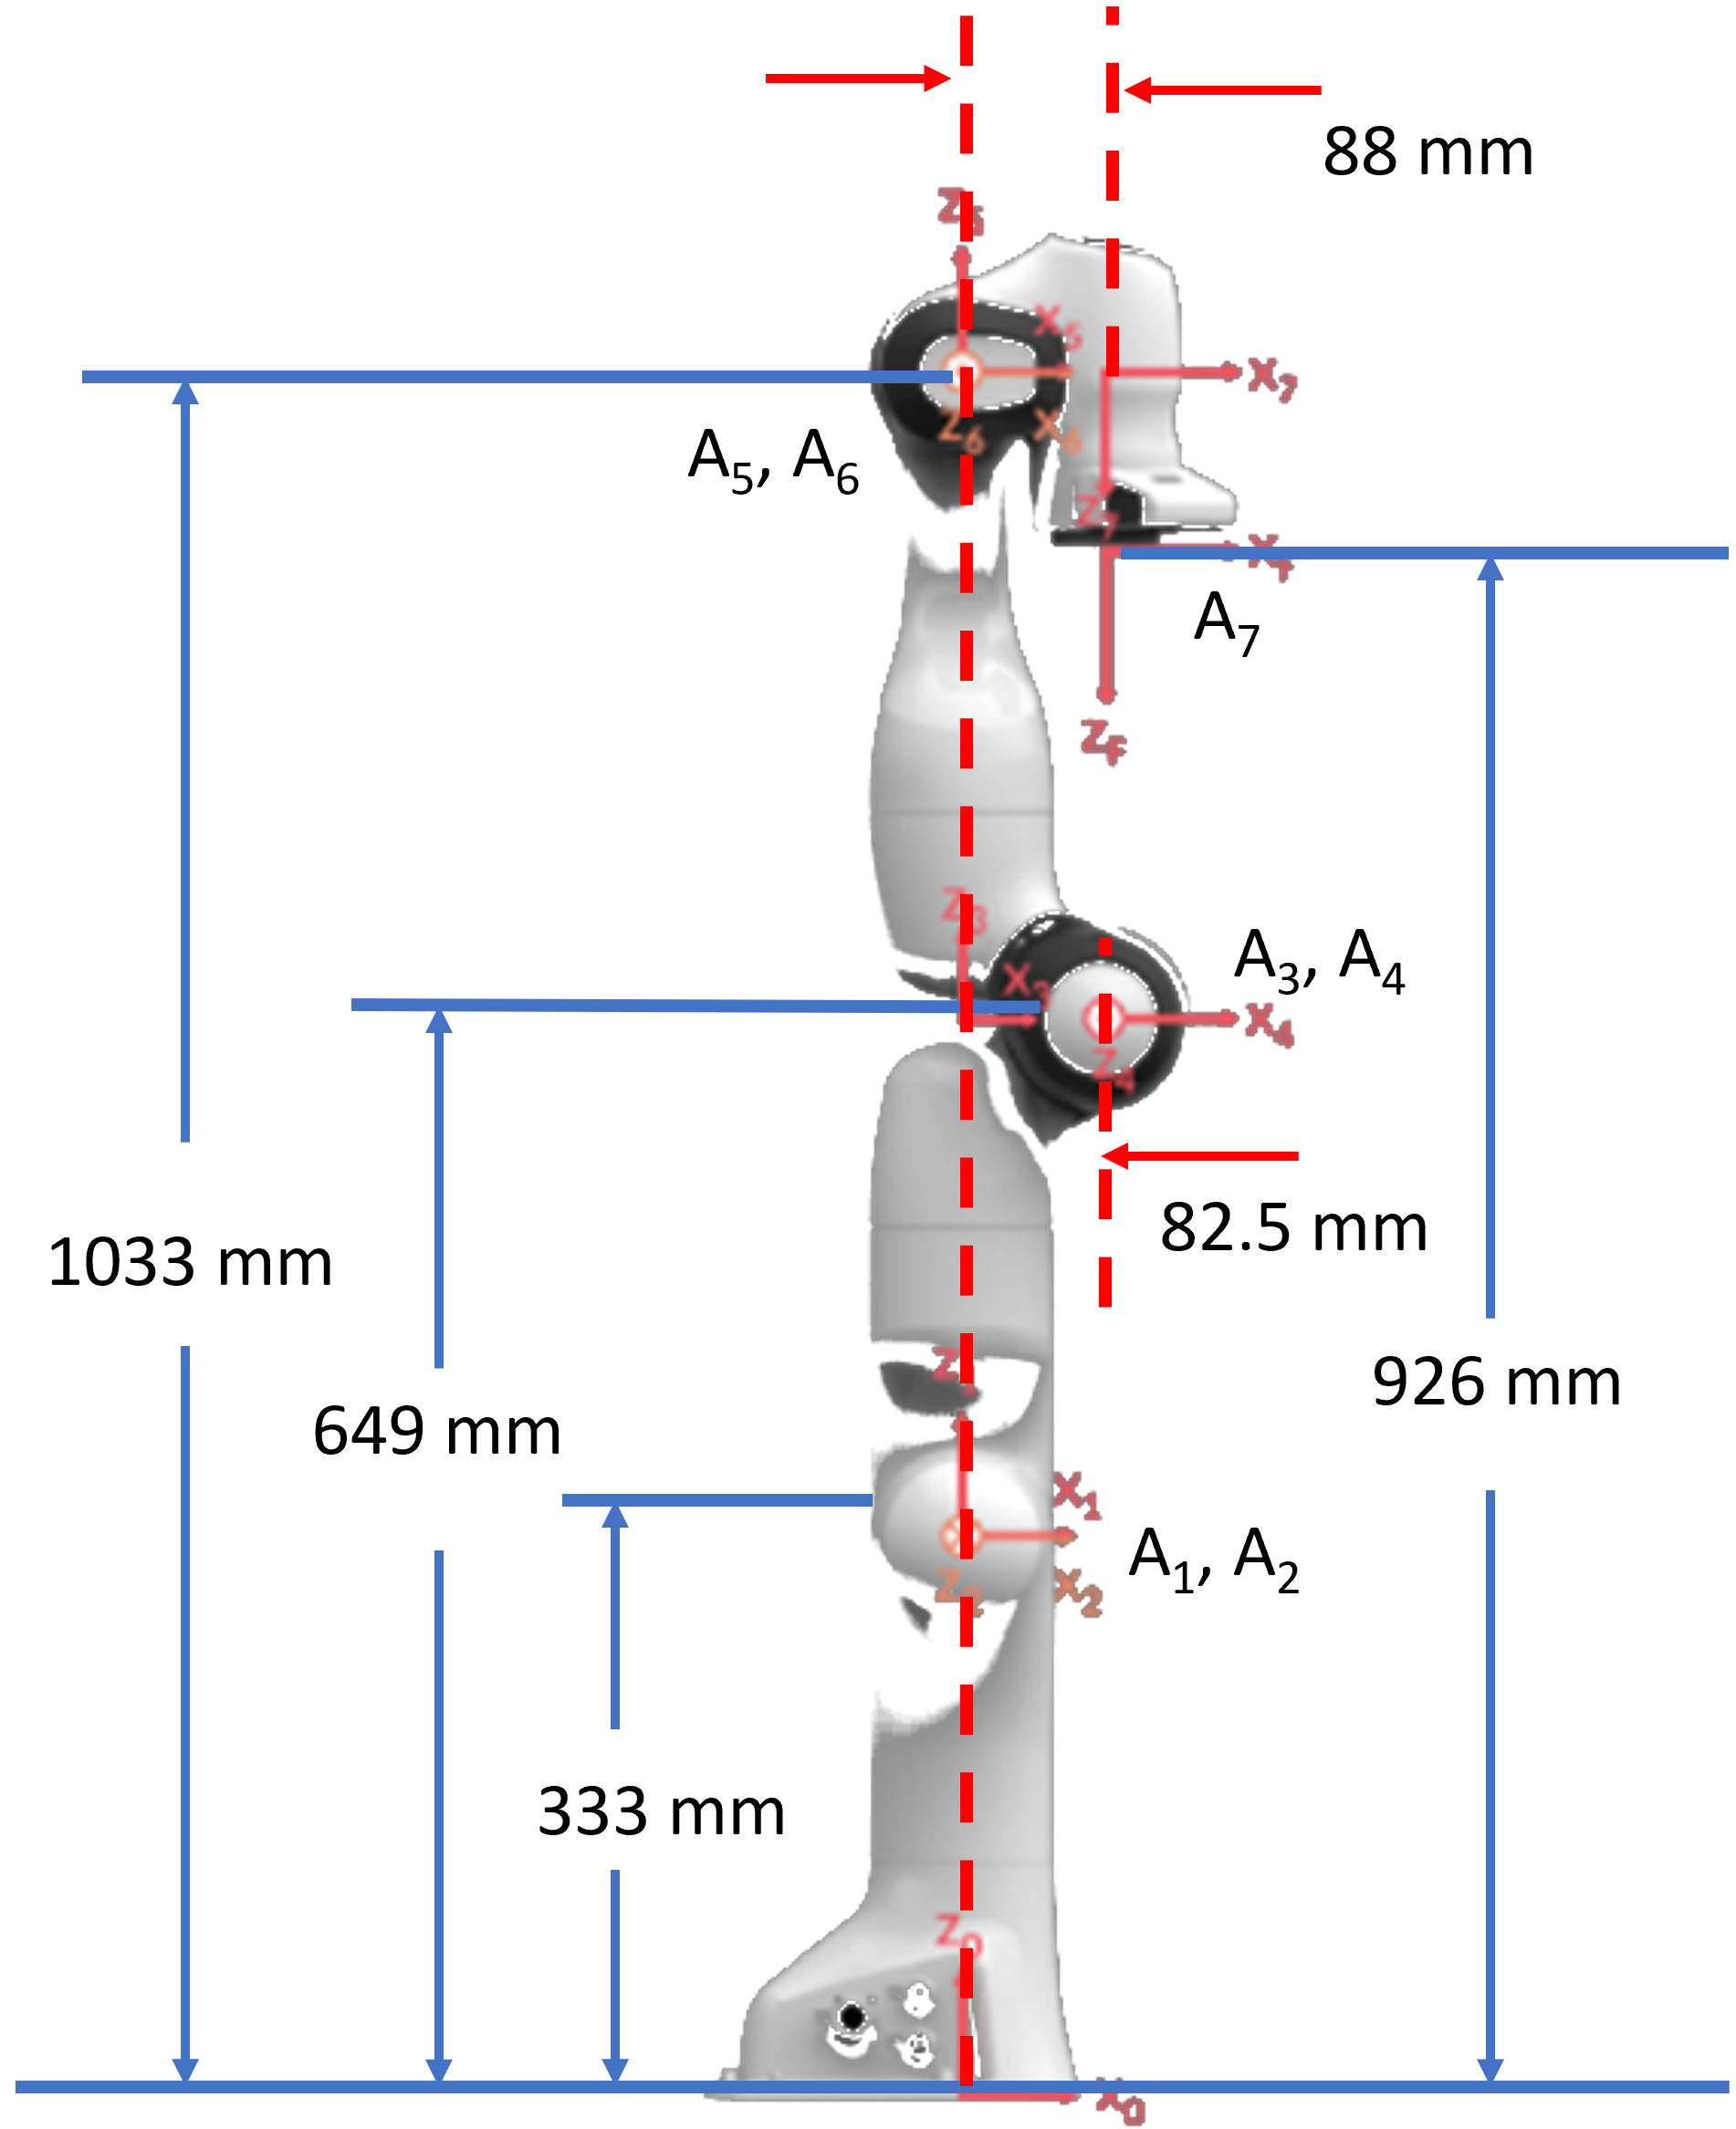
\includegraphics[scale=0.7]{dims.png}
        \caption{The parameters of Panda}
    \end{figure}
	
    The initial configuration is as follows:
    $$M = \begin{bmatrix}
        0 & 1 & 0 & 0.088\\
        1 & 0 & 0 & 0\\
        0 & 0 & -1 & 0.926 \\
        0 & 0 & 0 & 1 \\
    \end{bmatrix}$$
    
    Here is the twist for each joints.
    \begin{center}
        \begin{tabular}{|c|c|c|}
            \hline
            & $\omega_i$ & $v_i$ \\
            \hline
            A1 & $[0, 0, 1]^{T}$ & $[0, 0, 0]^{T}$ \\
            \hline
            A1 & $[0, 1, 0]^{T}$ & $[-0.333, 0, 0]^{T}$ \\
            \hline
            A3 & $[0, 0, 1]^{T}$ & $[0, 0, 0]^{T}$ \\
            \hline
            A4 & $[0, -1, 0]^{T}$ & $[0.649, 0, -0.0825]^{T}$ \\
            \hline
            A5 & $[0, 0, 1]^{T}$ & $[0, 0, 0]^{T}$ \\
            \hline
            A6 & $[0, -1, 0]^{T}$ & $[1.033, 0, 0]^{T}$ \\
            \hline
            A7 & $[0, 0, -1]^{T}$ & $[0, -0.088, 0]^{T}$ \\
            \hline
        \end{tabular}
    \end{center}
    
    Rotation angle restrictions
    \begin{center}
        \begin{tabular}{|c|c|c|}
            \hline
            & min$/^\circ$& max$/^\circ$ \\
            \hline
            A1 & -166 & 166 \\
            \hline
            A1 & -101 & 101 \\
            \hline
            A3 & -166 & 166 \\
            \hline
            A4 & -176 & -4 \\
            \hline
            A5 & -166 & 166 \\
            \hline
            A6 & -1 & 215 \\
            \hline
            A7 & -166 & 166 \\
            \hline
        \end{tabular}
    \end{center}
    
    \section{Programming Assignments}
    \subsection*{a) Find the FK of Panda using the space form of the exponential products}
	This is implemented in \textbf{FK\_space.m}. This function takes the initial configuration of the end-effector, the screw axes and the joint angles as pararmeters and output the coordinates of the end-effector. The declaration of the function is as follows:
    \begin{lstlisting}[style=matlab]
function [T] = FK_space(M, S, theta)
% FK_space calculates the configuration of the end-effector
% Inputs:
%     M is a matrix of 4x4 of initial configuration of end-effector
%     S is a matrix of 6xn of screw axes
%     theta is a joint angle vector nx1
% Outputs:
%   T   - 4x4 the configuration of the end-effector
    \end{lstlisting}
	
    The test program is called \textbf{FK\_space\_test.m}. In this program, we tested several cases of the Panda robot and compare it with the results from matlab robotics toolbox. (Note that the Panda in MATLAB robotics toolbox uses a different initial config of joint 7 with our config. Specifically, when we set the angle of joint 7 to be $-\pi/4$ and all other angles to be zero, we recover our initial configuration.)
	
    This is the screw axes for each joint of Panda
    \begin{center}
        \begin{tabular}{|c|c|}
            \hline
            &  S \\
            \hline
            A1 & $[0, 0, 1, 0, 0, 0]^{T}$ \\
            \hline
            A1 & $[0, 1, 0, -0.333, 0, 0]^{T}$ \\
            \hline
            A3 & $[0, 0, 1, 0, 0, 0]^{T}$ \\
            \hline
            A4 & $[0, -1, 0, 0.649, 0, -0.0825]^{T}$ \\
            \hline
            A5 & $[0, 0, 1, 0, 0, 0]^{T}$  \\
            \hline
            A6 & $[0, -1, 0, 1.033, 0, 0]^{T}$  \\
            \hline
            A7 & $[0, 0, -1, 0, 0.088, 0]^{T}$ \\
            \hline
        \end{tabular}
    \end{center}
    \subsubsection*{Case 1: Benchmark (Alough it is not feasible due to the angle constraint of joint 4)}
    We set $\theta = \begin{bmatrix}
        0 & 0 & 0 & 0 & 0 & 0 & 0
    \end{bmatrix}^T$. In this case, the configuration should be the initial configuration and it is.
    \subsubsection*{Case 2}
    We set $\theta = \begin{bmatrix}
        0 & -40^o & 0 & -110^o & 0 & 90^o & 0
    \end{bmatrix}^T$. In this case, we try to recover the case in \ref{joints}. Again, we got the same configuration with the MATLAB robotics toolbox.
    $$T = \begin{bmatrix}
        0 & 0.9397 & 0.3420 & 0.312 \\ 1 & 0 & 0 & 0\\ 0 & 0.3420 & -0.9397 & 0.7665\\ 0 & 0 & 0 & 1
    \end{bmatrix}$$
    This is a visualization using MATLAB robotics toolbox.
    \begin{figure}[H]
        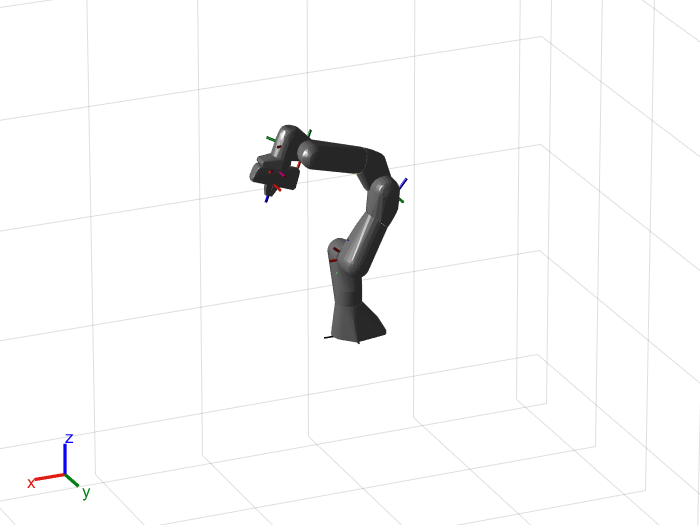
\includegraphics[scale=0.7]{p1t2.png}
    \end{figure}
    
    \subsubsection*{Case 3}
    We set $\theta = \begin{bmatrix}
        20^o & -40^o & 30^o & -110^o & -25^o & 90^o & 10^o
    \end{bmatrix}^T$. This is just a random case to test the rotation along $z$ axis (odd number joints). Again, we got the same configuration with the MATLAB robotics toolbox.
    $$T = \begin{bmatrix}
           -0.3041 &   0.6951  & 0.6515  &  0.1803 \\
        0.7230 &   0.6137 &  -0.3173  &  0.3012\\
        -0.6204  &  0.3745  & -0.6891  &  0.7456\\
        0      &   0     &    0  &  1.0000\\
    \end{bmatrix}$$
    This is a visualization using MATLAB robotics toolbox.
    \begin{figure}[H]
        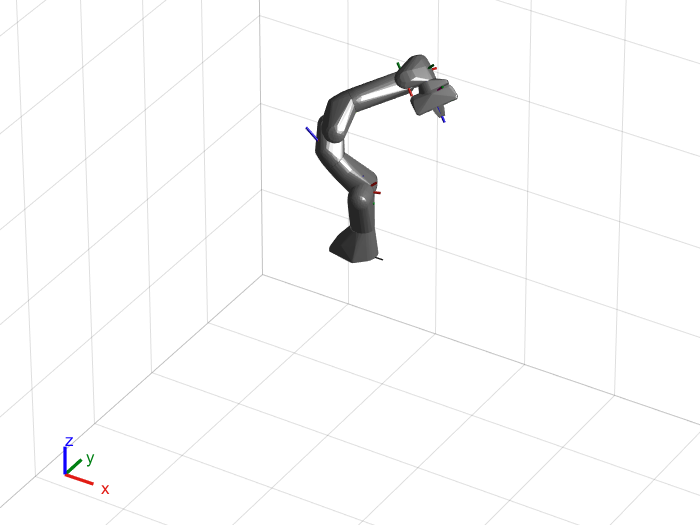
\includegraphics[scale=0.7]{p1t3.png}
    \end{figure}
	
    \subsection*{b) Calculate the space form FK of Panda and represent the defined frames and screw axis graphically}
    This is implemented in \textbf{visualize\_FK\_space.m} (instead of \textbf{FK\_space.m}, because \textbf{FK\_space.m} will be used later for many times to calculate the configuration of the end-effector and we think it is annoyting to plot the graph every time we call the function to get the end-effector).
	
    This function takes the initial configuration of the end-effector, the screw axes, the initial rotation directions, the initial joint positions and the joint angles. The declaration of the function is as follows:
    \begin{lstlisting}[style=matlab]
function visualize_FK_space(M, S, omega, r, theta)
% FK_space calculates the configuration of the end-effector
% Inputs:
%     M is a matrix of 4x4 of initial configuration of end-effector
%     S is a matrix of 6xn of screw axes
%     omega is a matrix of 3xn of initial rotation directions
%     r is a matrix of 3xn of initial joint positions
%     theta is a joint angle vector nx1
% Outputs:
%   T   - 4x4 the configuration of the end-effector
    \end{lstlisting}
    This function does pretty much the same thing with \textbf{FK\_space.m} except it plots the screw axes of each joint at configuration specified by parameter \textbf{theta}.
	
    In the test program \textbf{visualize\_FK\_space\_test.m}. We tested \textbf{Case 2} where \ \ \ $\theta = \begin{bmatrix}
        0 & -40^o & 0 & -110^o & 0 & 90^o & 0
    \end{bmatrix}^T$. Here is the graph generated by it compared with the MATLAB robotics toolbox.
    \begin{figure}[H]
        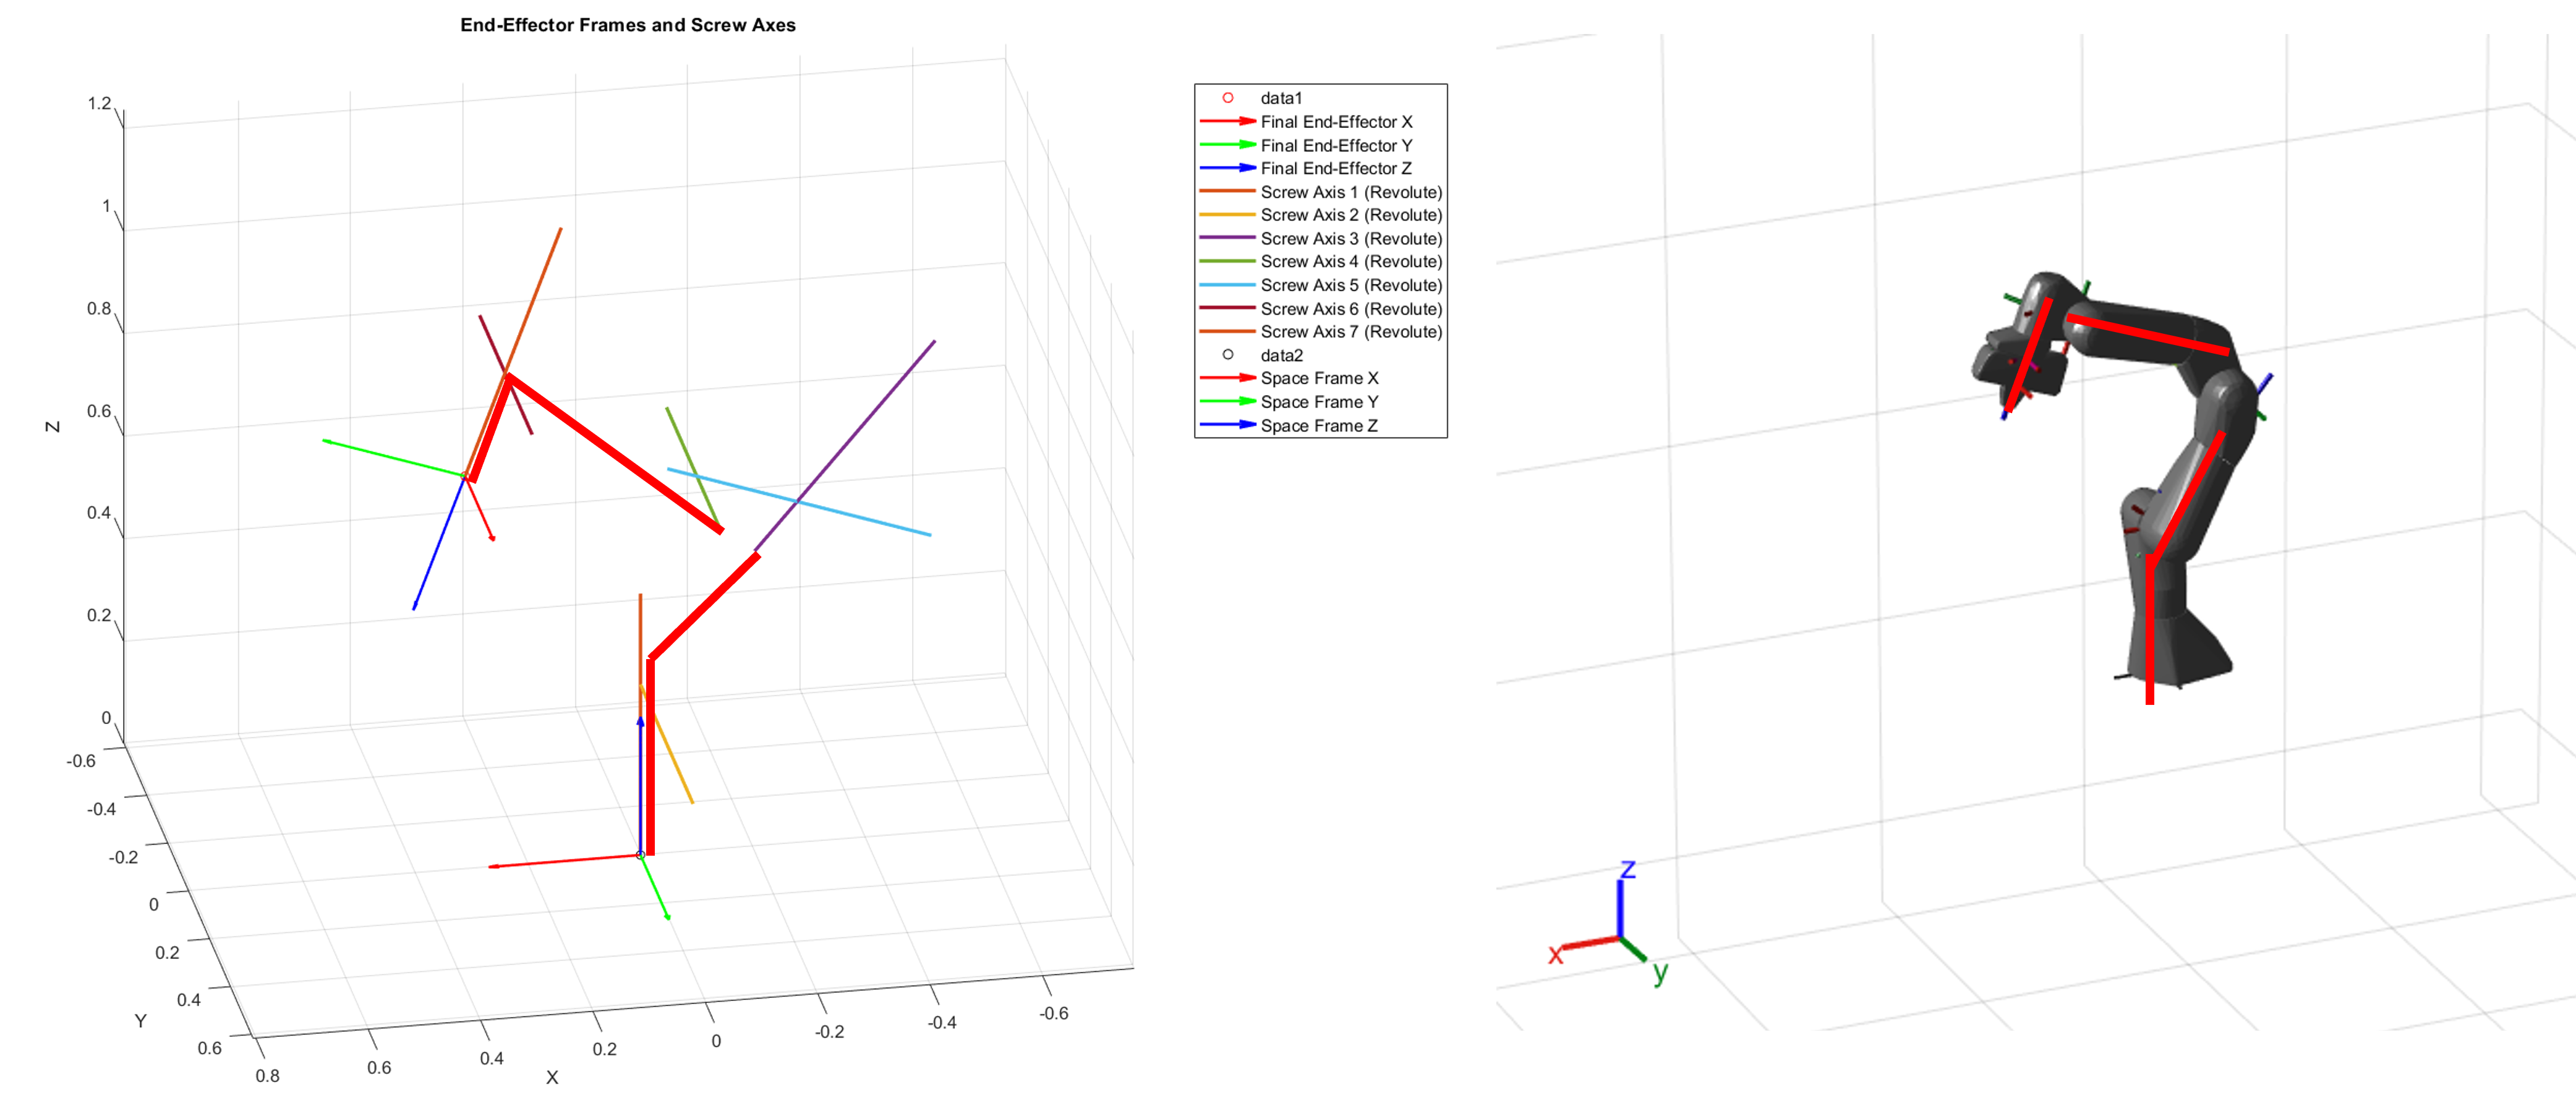
\includegraphics[scale=0.5]{p2t1.png}
    \end{figure}
    \subsection*{c) Repeat (a) and (b) for body form FK}
    This is implemented in \textbf{FK\_body.m}. This function takes the initial configuration of the end-effector, the screw axes in body form and the joint angles as parameters and outputs the coordinates of the end-effector.
    
    This is the screw axes in body form for each joint of Panda
    \begin{center}
        \begin{tabular}{|c|c|}
            \hline
            &  B \\
            \hline
            A1 & $[0, 0, -1, 0.088, 0, 0]^{T}$ \\
            \hline
            A1 & $[1, 0, 0, 0, 0.593, 0.088]^{T}$ \\
            \hline
            A3 & $[0, 0, -1, 0.088, 0, 0]^{T}$ \\
            \hline
            A4 & $[-1, 0, 0, 0, -0.277, -0.0055]^{T}$ \\
            \hline
            A5 & $[0, 0, -1, 0.088, 0, 0]^{T}$  \\
            \hline
            A6 & $[-1, 0, 0, 0, 0.1070, -0.088]^{T}$  \\
            \hline
            A7 & $[0, 0, 1, 0, 0, 0]^{T}$ \\
            \hline
        \end{tabular}
    \end{center}
	
    The test program is called \textbf{FK\_body\_test.m} where the three cases in \textbf{FK\_space\_test.m} were used and validated against the results here.
    
    Similarly, we have the \textbf{visualize\_FK\_body.m} to plot the defined frames and screw axes graphically and the corresponding test program \textbf{visualize\_FK\_body\_test.m} and we get the same results.
    
    \subsection*{d) Find the space and body form Jacobian of Panda}
    We use formulae

    $$\mathcal{V}_s = \begin{bmatrix}
    J_{s1} & J_{s2} & \cdots & J_{sn} 
\end{bmatrix}  \begin{bmatrix}
\dot{\theta}_1 \\ \dot{\theta}_2 \\ \vdots \\ \dot{\theta}_n
\end{bmatrix}$$
    where 
\begin{align*}
    J_{s1} &= \mathcal{S}_1 \\
    J_{s2} &= \text{Ad}_{e^{[S_1]\theta_1}} \mathcal{S}_2 \\
    \cdots
\end{align*}

    Similarly, for body form Jacobian:
$$\mathcal{V}_b = \begin{bmatrix}
    J_{b1} & J_{b2} & \cdots & J_{bn} 
\end{bmatrix}  \begin{bmatrix}
    \dot{\theta}_1 \\ \dot{\theta}_2 \\ \vdots \\ \dot{\theta}_n
\end{bmatrix}$$
    where 
\begin{align*}
    J_{bn} &= \mathcal{B}_n \\
    J_{b,{n-1}} &= \text{Ad}_{e^{-[B_n]\theta_n}} \mathcal{B}_{n-1} \\
    \cdots
\end{align*}
	
    \subsection*{e) Write functions to calculate the space and body form Jacobians of the robot}
These are implemented in \textbf{J\_space.m} and \textbf{J\_body.m} for space and body form Jacobians, respectively. For the space-form Jacobian, the function takes the screw axes in body form and the joint angles as parameters and outputs the space-form Jacobian of the end-effector. The declaration of the function is as follows:
    \begin{lstlisting}[style=matlab]
function [J] = J_space(S, theta)
% J_SPACE Calculate the space Jacobian matrix for a serial robot
%
% Inputs:
%   S     - 6xn matrix of normalized twists, where each column is a 6x1 twist
%          vector [omega; v] representing the joint axis in space frame
%   theta - nx1 vector of joint angles/positions
%
% Output:
%   J     - 6xn space Jacobian matrix
\end{lstlisting}
    The body form of the Jacobian is similar.
    \subsubsection*{Case 1-3}
    The test program is called \textbf{J\_space\_body\_test.m} to test the two functions. Again, we used the three cases mentioned earlier. The test is two-fold. Firstly, we use cross-validation of the space-form Jacobian and body-form Jacobian with the following formulae:
    \[J_s = \text{Ad}_{T_{sb}} J_b\]
    Secondly, we validate our results with the results from MATLAB robotics toolbox. Note that the Jacobian calculated by \textbf{geometricJacobian} is actually analytic form Jacobian, as stated in \cite{Lynch_Park_2017}. And it can be transformed to body-form Jacobian using the following formulae:
    \[J_a = \begin{bmatrix}
        R_{sb} & 0 \\
        0 & R_{sb}
    \end{bmatrix} J_b\]
    \subsubsection*{Case 4}
    We further tested our program using the definition of Jacobian matrix.
    \begin{equation}
        J(\theta)\Delta \theta = \text{Ad}(\Delta T)
    \end{equation}
    or
    \begin{equation}
        J(\theta)\Delta \theta = \text{Ad}_{T(\theta + \Delta \theta) / T(\theta)}
    \end{equation}
    For example, when $\theta = \begin{bmatrix}
        0 & -40^o & 0 & -110^o & 0 & 90^o & 0
    \end{bmatrix}^T$ and $\Delta\theta$ is chosen to be \ \ \ $\theta = \pi/200\begin{bmatrix}
        1 & 1 & 1 & 1 & 1 & 1 & 1
    \end{bmatrix}^T$. We get
    \begin{equation}
        \text{Ad}_{T(\theta + \Delta \theta) / T(\theta)} = \begin{bmatrix}
                0.0106 &   -0.0154 &   0.0185 &   0.0175 &   0.0172 &  -0.0009
        \end{bmatrix}^T
    \end{equation}
    And 
    \begin{equation}
        J(\theta)\Delta \theta = \begin{bmatrix}
                0.0100 &   -0.0157 &   0.0184 &   0.0178 &   0.0167 &  -0.0008
        \end{bmatrix}^T
    \end{equation}
    which are very close, as expected.
    \subsection*{f) Write a function \textbf{singularity.m} to calculate the singularity configurations of the robot}
    According to \cite{Hepanda} and \cite{Tittelpanda}, Panda's singularity exists when joints 1, 3 and 5 aligned and the robot would lose two DoF, leaving it with just 5-DoF and incapable of certain motion. It is acchieved when $\theta = \begin{bmatrix}
        0 & 0 & 0 & 0 & 0 & 0 & 0
    \end{bmatrix}^T$, as shown in the following picture. 
    \begin{figure}[H]
        \centering
        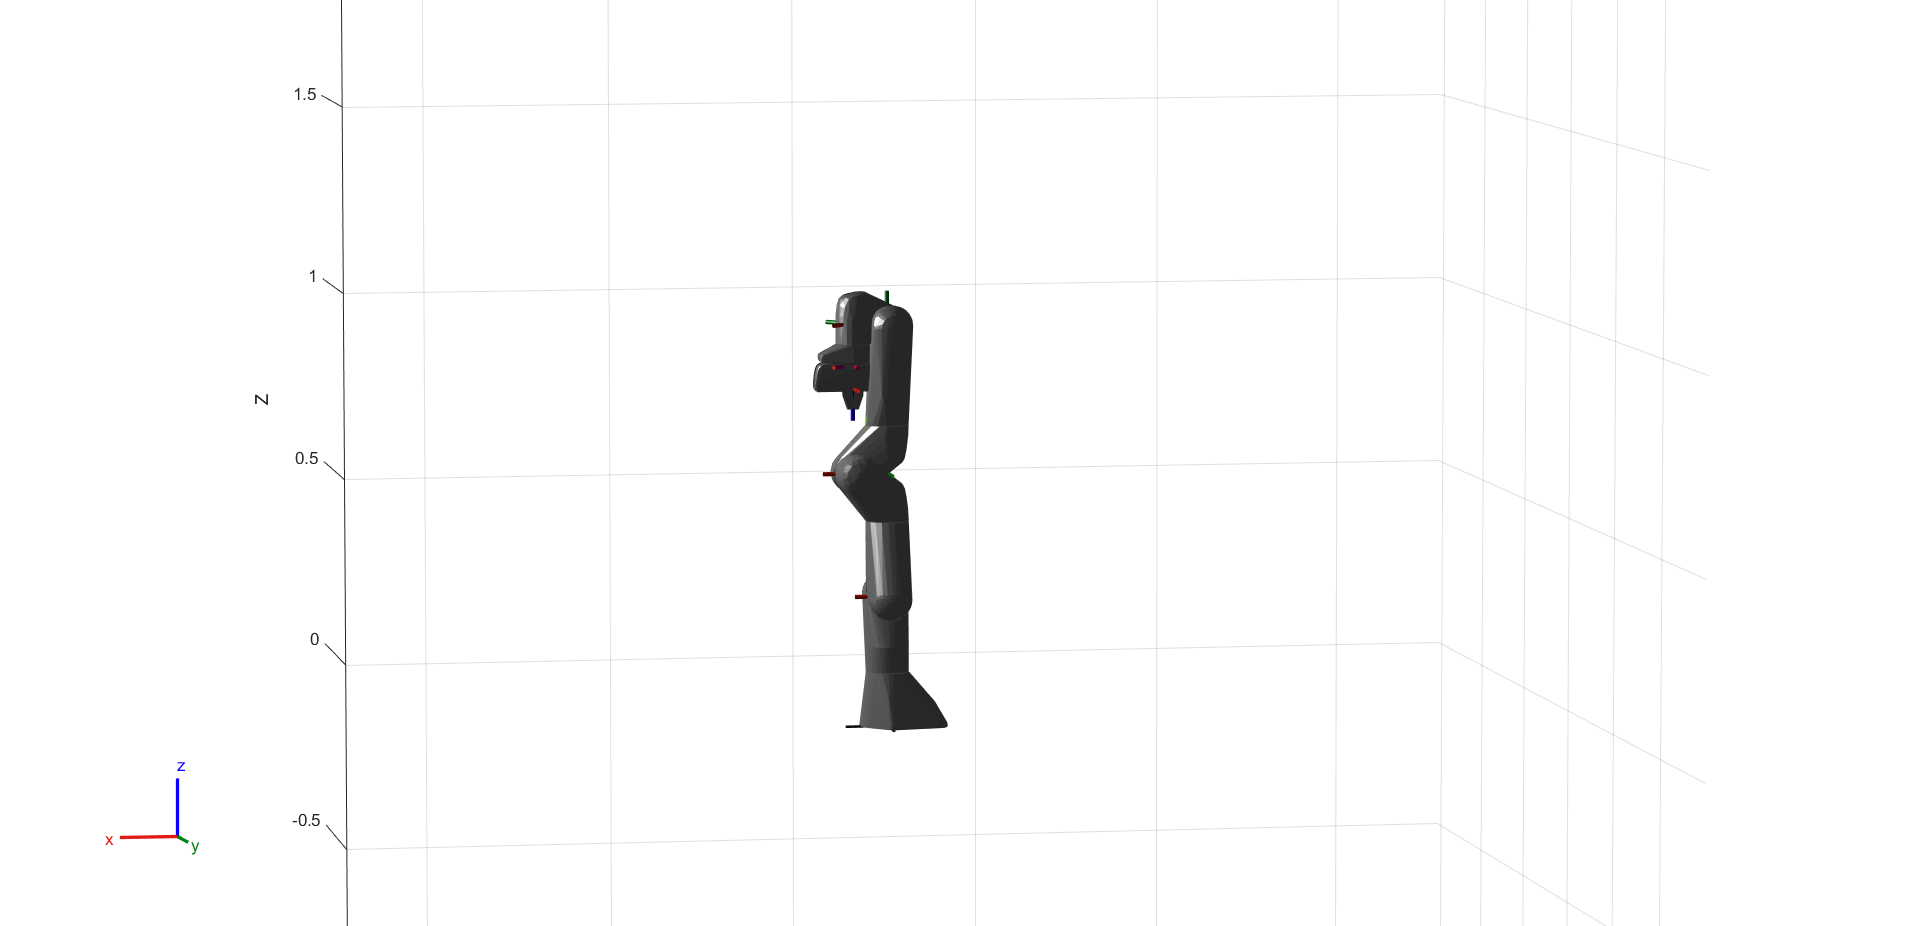
\includegraphics[width=\linewidth]{singularity.png}
        \caption{Singularity case}
        \label{fig:enter-label}
    \end{figure}
    This could be validated using the rank of Jacobian matrix. Furthermore, we can use function \textbf{jsingu} to show which columns are linearly dependent.
    \begin{lstlisting}[style=matlab]
         5

2 linearly dependent joints:
  q3 depends on: q1 
  q5 depends on: q1 
    \end{lstlisting}

    \subsection*{g) Write functions that }
    \subsubsection*{a) show/plot the manipulability ellipsoids for the angular and linear velocities and their axes}
    The two functions are implemented in \textbf{ellipsoid\_plot\_angular.m} and \textbf{ellipsoid\_plot\_linear.m}, respectively. And their test program with sufix \textbf{\_test}.
    
    When $\theta = \begin{bmatrix}
        0 & 0 & 0 & 0 & 0 & 0 & 0
    \end{bmatrix}^T$, we know it is at singularity and the ellipsoid should be a plane for angular velocities. (Because we lost the freedom in angular motions instead of linear motions) And so did our program got.
    \begin{figure}[H]
        \centering
        \begin{minipage}{0.45\textwidth}
            \centering
            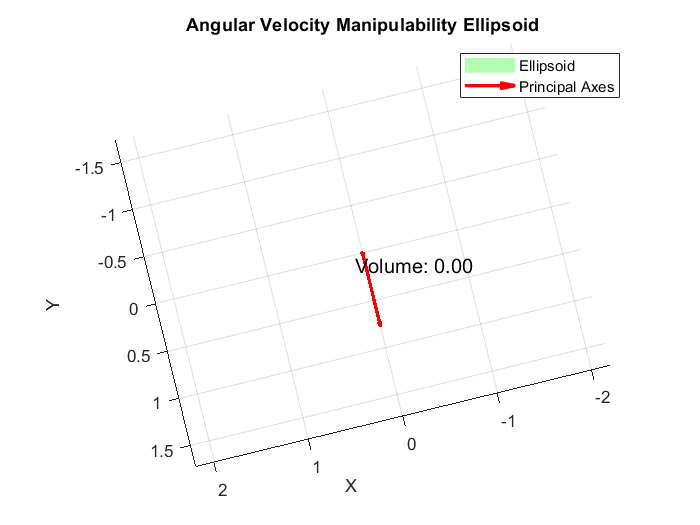
\includegraphics[width=\textwidth]{pga1a.png} % Replace with your image file
            \caption{Angular Velocity Manipulability Ellipsoid}
            \label{fig:pga1a}
        \end{minipage}
        \hfill
        \begin{minipage}{0.45\textwidth}
        \centering
            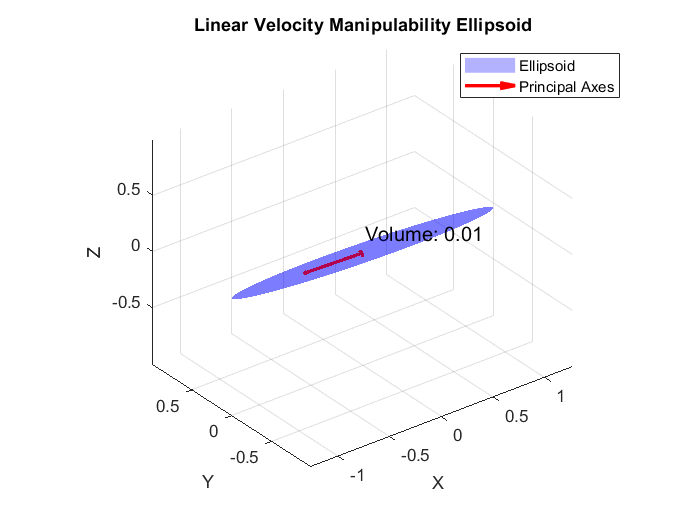
\includegraphics[width=\textwidth]{pga1l.png} % Replace with your image file
            \caption{Linear Velocity Manipulability Ellipsoid}
            \label{fig:pga1l}
        \end{minipage}
    \end{figure}

    The following are the results when $\theta = \begin{bmatrix}
        0 & -40^o & 0 & -110^o & 0 & 90^o & 0
    \end{bmatrix}^T$ which is not at singularity.
    \begin{figure}[H]
        \centering
        \begin{minipage}{0.45\textwidth}
            \centering
            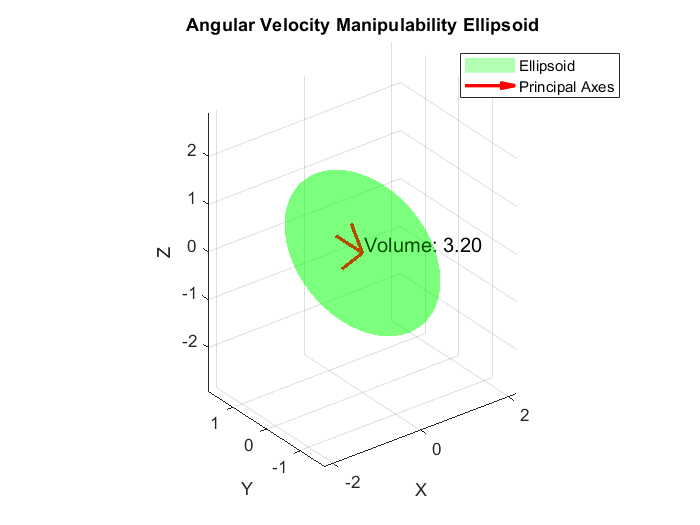
\includegraphics[width=\textwidth]{pga2a.png} % Replace with your image file
            \caption{Angular Velocity Manipulability Ellipsoid}
            \label{fig:pga2a}
        \end{minipage}
        \hfill
        \begin{minipage}{0.45\textwidth}
        \centering
            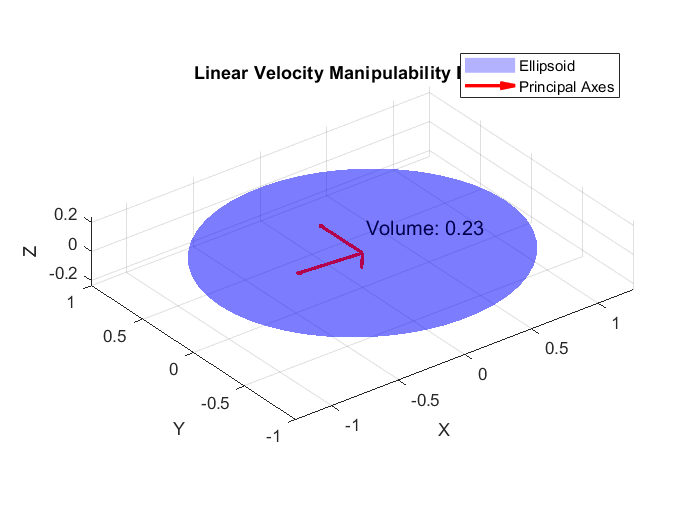
\includegraphics[width=\textwidth]{pga2l.png} % Replace with your image file
            \caption{Linear Velocity Manipulability Ellipsoid}
            \label{fig:pga2l}
        \end{minipage}
    \end{figure}
    \subsubsection*{b) Calculate the isotropy, condition number and volume of the ellipsoids}
    \begin{table}[h]
    \centering
    \begin{tabular}{|p{1.5cm}|c|c|c|c|}
        \hline
        \multirow{2}{*}{ } & \multicolumn{2}{|c|}{Case 1\newline \(\theta = \begin{bmatrix}
        0 & 0 & 0 & 0 & 0 & 0 & 0 \end{bmatrix}^T\)} & \multicolumn{2}{|c|}{Case 2 $\theta = \begin{bmatrix}
        0 & -40^o & 0 & -110^o & 0 & 90^o & 0
    \end{bmatrix}^T$} \\ \cline{2-5}
         &  space-form Jacobian & body-form Jacobian & space-form Jacobian & body-form Jacobian\\ \hline
        isotropy & Inf & Inf & 10.90 & 9.75 \\ \hline
        condition number & Inf & Inf & 118 & 95 \\ \hline
        volume of the ellipsoid & 0 & 0 & 0.0929 & 0.0929 \\ \hline
    \end{tabular}
    \caption{test results for isotropy, condition number and volume of the ellipsoids}
    \label{tab:pgb}
    \end{table}
    From the test results, we observe that 
    \begin{enumerate}
        \item when \(\theta = \begin{bmatrix}
        0 & 0 & 0 & 0 & 0 & 0 & 0 \end{bmatrix}^T\), the robot is at singularity. Therefore, the isotropy and condition number is infinity which is as expected.
        \item when \(\theta = \begin{bmatrix} 0 & -40^o & 0 & -110^o & 0 & 90^o & 0 \end{bmatrix}^T\), the isotropy and condition number are greater than 1. The volume by calculated by space-form Jacobian and body-form Jacobian are the same.
    \end{enumerate}

    \subsection*{h) Use the derived forward kinematics and Jacobians, write a function that uses the iterative numerical inverse kinematics algorithm to control the robot from arbitrary configuration a to configuration b}
    Here, we used the space-form Jacobian to conduct inverse kinematics. The update formulae is
    \begin{align}
        error &= \text{Ad}_{T_{sb}} [T_{sb} \ T_{sd}]\\ \nonumber
        \theta &= \theta + J^\dagger error
    \end{align}
    The declaration of the function is as follows:
    \begin{lstlisting}[style=matlab]
function theta = J_inverse_kinematics(M, S, T_desired, theta_init, epsilon)
% J_inverse_kinematics Solve inverse kinematics using iterative Newton-Raphson method
%
% Inputs:
%   B          - 6xn matrix of normalized twists in body frame
%   M          - 4x4 home configuration matrix
%   T_desired  - 4x4 desired end-effector configuration matrix
%   theta_init - nx1 initial guess for joint angles
%   epsilon    - Error tolerance (default: 1e-4)
%
% Outputs:
%   theta   - nx1 vector of joint angles that achieve T_desired
%   success - Boolean indicating whether algorithm converged
%
% Note:
%   Uses Newton-Raphson iteration with space Jacobian.
    \end{lstlisting}
    The test program is called \textbf{J\_inverse\_kinematics\_test.m} to test the function.
    \subsection*{Case 1}
    In this case, we set $T_{sd}$ (which is random)
    \begin{equation}
        T_{sd} = \begin{bmatrix}
            0.3862 & -0.2690 & -0.8823 & 0.4225\\
            0.8917 & 0.3535 & 0.2826 & 0.3776\\
            0.2359 & -0.8959 & 0.3764 &  -0.0874\\
            0 & 0 & 0 & 1.00
        \end{bmatrix}
    \end{equation}
    And we use random initial \(\theta = \begin{bmatrix}
        0 & -\pi/2 & 0 & -\pi/2 & 0 & 0 & 0 \end{bmatrix}^T\). (Note to keep to within the joint angle constraints). The followings pictures shows the initial and desired configuration of the robot.
    \begin{figure}[H]
        \centering
        \begin{minipage}{0.45\textwidth}
            \centering
            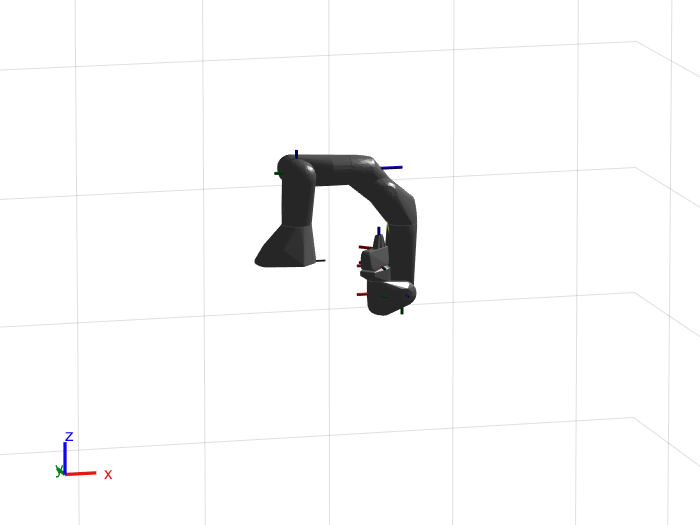
\includegraphics[width=\textwidth]{ph1a.png} % Replace with your image file
            \caption{Initial Configuration}
            \label{fig:ph1a}
        \end{minipage}
        \hfill
        \begin{minipage}{0.45\textwidth}
        \centering
            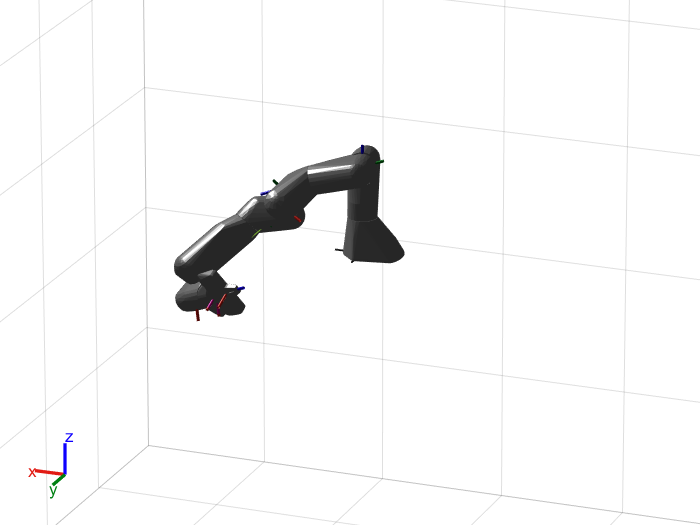
\includegraphics[width=\textwidth]{ph1b.png} % Replace with your image file
            \caption{Desired Configuration}
            \label{fig:ph1b}
        \end{minipage}
    \end{figure}
    This program output \(\theta = \begin{bmatrix} 0.5642 & 1.8297 & -0.1648 & -0.6123 & 1.3935 & 0.7434 & 0.4404 \end{bmatrix}^T\) and exactly the same final configuration of the end-effector.
    
    \subsection*{Case 2}
    In this case, we test the robustness of the program by setting the desired configuration to be very close to singularity. (\(\theta = \begin{bmatrix}
        0.01 & 0.02 & 0.03 & -0.1 & 0.05 & 0.06 & 0.07 \end{bmatrix}^T\)) The desired configuration is
    \begin{equation}
        T_{sd} = \begin{bmatrix}
            -0.0198 & 0.9980 & -0.0601 & 0.1339\\
            0.9998 & 0.0199 & 0.0012 & 0.0097\\
            0.0024 & -0.0601 & -0.9982 & 0.9263\\
            0 & 0 & 0 & 1.00
        \end{bmatrix}
    \end{equation}
    And the condition number at this place is \(1621.7\).
    
    And we use initial guess \(\theta = \begin{bmatrix}
        0 & 1 & 0 & -0.5 & 0 & 0 & 0 \end{bmatrix}^T\). The followings pictures shows the initial and desired configuration of the robot.
    \begin{figure}[H]
        \centering
        \begin{minipage}{0.45\textwidth}
            \centering
            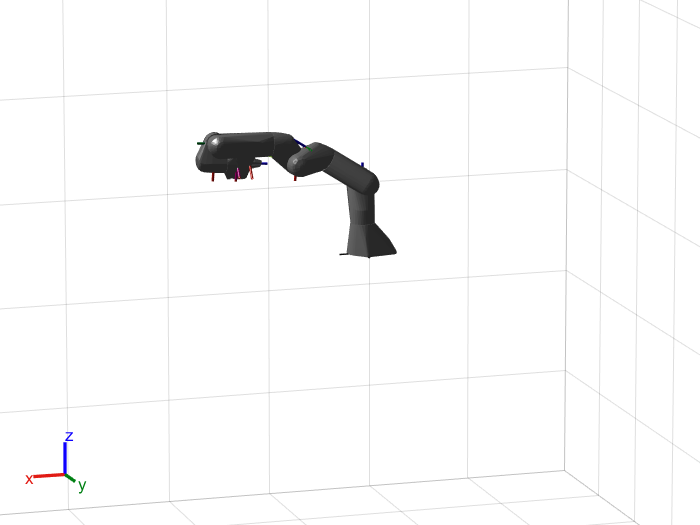
\includegraphics[width=\textwidth]{ph2a.png} % Replace with your image file
            \caption{Initial Configuration}
            \label{fig:ph2a}
        \end{minipage}
        \hfill
        \begin{minipage}{0.45\textwidth}
        \centering
            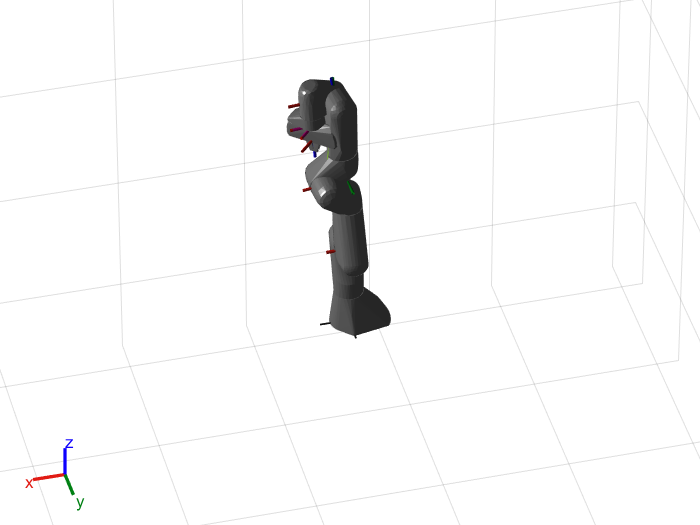
\includegraphics[width=\textwidth]{ph2b.png} % Replace with your image file
            \caption{Desired Configuration}
            \label{fig:ph2b}
        \end{minipage}
    \end{figure}
    This program output exactly the same final configuration of the end-effector and \ \ \ \(\theta = \begin{bmatrix} -3.2855 & 12.1961 & 5.6213 & 18.3704 & 2.4528 & -6.5735 & 4.8143 \end{bmatrix}^T\). The \(\theta\) exceeds the joint angles limits and needed further modification.

    \subsection*{i) Use Jacobian Transpose algorithm}
    Again, we used the space-form Jacobian to conduct transpose kinematics. According to \cite{ik}, the update formulae is 
    \begin{align}
        e &= \text{Ad}_{T_{sb}} [T_{sb} \ T_{sd}]\\ \nonumber
        \theta &= \theta + \alpha J^T e \\
        \alpha &= \frac{<e, JJ^Te>}{<JJ^Te, JJ^Te>}
    \end{align}
    
    We used the two cases introduced in \textbf{J\_inverse\_kinematics\_test.m} test the function in \textbf{J\_transpose\_kinematics\_test.m}
    \subsection*{Case 1}
    In this case, we set $T_{sd}$
    \begin{equation}
        T_{sd} = \begin{bmatrix}
            0.3862 & -0.2690 & -0.8823 & 0.4225\\
            0.8917 & 0.3535 & 0.2826 & 0.3776\\
            0.2359 & -0.8959 & 0.3764 &  -0.0874\\
            0 & 0 & 0 & 1.00
        \end{bmatrix}
    \end{equation}
    This program outputs \(\theta = \begin{bmatrix} 0.3642 & 1.8267 & 0.3159 & -0.6573 & 0.8888 & 0.8956 & 0.4970 \end{bmatrix}^T\) and exactly the same final configuration of the end-effector.

    \subsection*{Case 2}
    In this case, the desired configuration is
    \begin{equation}
        T_{sd} = \begin{bmatrix}
            -0.0198 & 0.9980 & -0.0601 & 0.1339\\
            0.9998 & 0.0199 & 0.0012 & 0.0097\\
            0.0024 & -0.0601 & -0.9982 & 0.9263\\
            0 & 0 & 0 & 1.00
        \end{bmatrix}
    \end{equation}
    This program output exactly the same final configuration of the end-effector and \ \ \ \ \ \(\theta = \begin{bmatrix} 0.0046 & 0.0208 & 0.0369 & -0.0985 & 0.0491 & 0.0593 & 0.0707 \end{bmatrix}^T\), which is a much better result than \textbf{J\_inverse\_kinematics.m}
    
    \subsection*{j) Use the redundancy resolution approach to maximize the manipulability and exploit redundancy to move away from singularities}
    We use volume of the manipulability ellipsoids as the second objective function.
    \begin{align}
    	\theta &= \theta + J^\dagger e + \alpha N \nabla V\\ \nonumber
    	V &= \sqrt{\det(J J^T)} \\
    	N &= I - J^\dagger J
    \end{align}
	
	Here, we choose $\alpha = 0.1$
	\subsection*{Case 1}
	In this case, we set $T_{sd}$
	\begin{equation}
		T_{sd} = \begin{bmatrix}
			0.3862 & -0.2690 & -0.8823 & 0.4225\\
			0.8917 & 0.3535 & 0.2826 & 0.3776\\
			0.2359 & -0.8959 & 0.3764 &  -0.0874\\
			0 & 0 & 0 & 1.00
		\end{bmatrix}
	\end{equation}
	This program outputs \(\theta = \begin{bmatrix} 0.5631 & 1.8295 & -0.1622 & -0.6124 & 1.3906 & 0.7442 & 0.4405 \end{bmatrix}^T\) and exactly the same final configuration of the end-effector.
	
	\subsection*{Case 2}
	In this case, the desired configuration is
	\begin{equation}
		T_{sd} = \begin{bmatrix}
			-0.0198 & 0.9980 & -0.0601 & 0.1339\\
			0.9998 & 0.0199 & 0.0012 & 0.0097\\
			0.0024 & -0.0601 & -0.9982 & 0.9263\\
			0 & 0 & 0 & 1.00
		\end{bmatrix}
	\end{equation}
	This program output exactly the same final configuration of the end-effector and \ \ \ \ \ \(\theta = \begin{bmatrix} -3.3297 & 12.1911 & 5.6309 & 18.3437 & 2.4948 & -6.5875 & 4.8244 \end{bmatrix}^T\), which is a very close to the result from \textbf{J\_inverse\_kinematics.m} and not a reasonable result.
	
    \subsection*{h) Extend the inverse kinematics utilizing the Damped Least Square Approach}
    We use the volume of the manipulability ellipsoids as judging criterion, when the volume is large (larger than 0.01 in our program) we stick to the method in \textbf{J\_inverse\_kinematics.m}. Otherwise, the update formulae is switched to
    \begin{align}
        \theta &= \theta + J ^T ( J J^T + k^2 I) e 
    \end{align}
    
    \subsection*{Case 1}
    In this case, we set $T_{sd}$
    \begin{equation}
        T_{sd} = \begin{bmatrix}
            0.3862 & -0.2690 & -0.8823 & 0.4225\\
            0.8917 & 0.3535 & 0.2826 & 0.3776\\
            0.2359 & -0.8959 & 0.3764 &  -0.0874\\
            0 & 0 & 0 & 1.00
        \end{bmatrix}
    \end{equation}
    This program outputs \(\theta = \begin{bmatrix} 0.5642 & 1.8297 & -0.1648 & -0.6123 & 1.3935 & 0.7434 & 0.4404 \end{bmatrix}^T\) which is exactly the same with the result from \textbf{J\_inverse\_kinematics.m}. This is because in this case, the robot is far from the singularity. Therefore, it works exactly the same with \textbf{J\_inverse\_kinematics.m}.

    \subsection*{Case 2}
    In this case, the desired configuration is
    \begin{equation}
        T_{sd} = \begin{bmatrix}
            -0.0198 & 0.9980 & -0.0601 & 0.1339\\
            0.9998 & 0.0199 & 0.0012 & 0.0097\\
            0.0024 & -0.0601 & -0.9982 & 0.9263\\
            0 & 0 & 0 & 1.00
        \end{bmatrix}
    \end{equation}
    This program output exactly the same final configuration of the end-effector and \ \ \ \ \ \(\theta = \begin{bmatrix} 0.0195 & 0.0206 & 0.0182 & -0.0989 & 0.0519 & 0.0595 & 0.0696 \end{bmatrix}^T\), which is a much better result than \textbf{J\_inverse\_kinematics.m}
    \printbibliography
\end{document}